\documentclass[11pt]{article}
\usepackage{classTools}
\usepackage{amsmath, amssymb}

\begin{document}

\psHeader{3}{Wed Oct. 2, 2024 (11:59pm)}

\textbf{Your name: Roshen Chatwal}

\textbf{Collaborators: Raunak Daga and ChatGPT (used for research into how Python handles bignums) }

\textbf{No. of late days used on previous psets: 0 days, 7 minutes }

\textbf{No. of late days used after including this pset: 0 days, maybe like 20 minutes if I'm not quick enough with it}


The purpose of this problem set is to solidify your understanding of the RAM model (and variants), and the relations between the RAM model, the Word-RAM model, Python programs, and variants. In particular, you will build skills in simulating one computational model by another and in evaluating the runtime of the simulations (both in theory and in practice).

\textit{Note: We STRONGLY recommend typing this problem set (in LaTeX, if possible) -- question 3 will probably be the longest proof we've had you write in the course so far, and unless you have typewriter handwriting, it is much easier for us to grade typed submissions. If we can't read your handwriting, chances are it will lose points.}

\begin{enumerate}
 
    \item (Simulation in practice: RAMs on Python)  
    In the Github repository, we have given you a partially written Python implementation of a universal RAM Model simulator.  Your task is to fill in the missing parts of the code to obtain a complete universal RAM simulator.
     Your simulator should take as input a RAM Program $P$ and an input $x$, and simulate the execution of $P$ on $x$, and return whatever output $P$ produces (if it halts).  The RAM Program $P$ is given as a Python list $[v,C_0,C_1,\ldots,C_{\ell-1}]$, where $v$ is the number of variables used by $P$.  For simplicity, we assume that the variables are named $0,\ldots,v-1$ (rather than having names like ``tmpptr'' and ``insertvalue''), but you can introduce constants to give names to the variables.  The $0$\textsuperscript{th} variable will always be $\inputlen$, the $1$\textsuperscript{st} variable $\outputpointer$, and the $2$\textsuperscript{nd} variable $\outputlen$.  A command $C$ is given in the form of a list of the form $[\cmd]$, $[\cmd,i]$, $[\cmd,i,j]$, or $[\cmd,i,j,k]$, where $\cmd$ is the name of the command and $i,j,k$ are the indices of the variables or line numbers used in the command.  For example,  the command $\var_i = M[\var_j]$ would be represented as $(\READ,i,j)$.  See the Github repository for the precise syntax as well as some RAM programs you can use to test your simulator.

    \item (Empirically evaluating simulation runtimes and explaining them theoretically)  

Consider the following two RAM programs:

\begin{algorithm}[H]
\Input{A single natural number $N$ (as an array of length 1)}
\Output{$13^{2^N+1}$ (as an array of length 1)}
\Variables{$\inputlen, \outputpointer, \outputlen, \counter, \result$}
\setcounter{AlgoLine}{-1}
$\zero = 0$\;
$\one = 1$\;
$\thirteen = 13$\;
$\outputlen = 1$\;
$\outputpointer = 0$\;
$\result = 13$\;
$\counter = M[\zero]$\;
\Indp
 IF $\counter == 0$ GOTO \ref{line:done}\; \label{line:loop}
$\result = \result \times \result$\;
$\counter = \counter - \one$\;
IF $\zero == 0$ GOTO \ref{line:loop}\;
\Indm
$\result = \result \times $\thirteen\; \label{line:done}
$M[\outputpointer]=\result$\;
\end{algorithm}

\begin{algorithm}[H]
\Input{A single natural number $N$ (as an array of length 1)}
\Output{$13^{2^N+1} \bmod 2^{32}$ (as an array of length 1)}
\Variables{$\inputlen, \outputpointer, \outputlen, \counter, \result, \temp, \W$}
\setcounter{AlgoLine}{-1}
$\zero = 0$\;
$\one = 1$\;
$\thirteen = 13$\;
$\outputlen = 1$\;
$\outputpointer = 0$\;
$\result = 13$\;
$\W = 2^{32}$\;
$\counter = M[\zero]$\;
\Indp
IF $\counter == 0$ GOTO \ref{line:done2}\; \label{line:loop2}
$\result = \result \times \result$\;
$\temp = \result / \W$\;
$\temp = \temp \times \W$\;
$\result = \result - \temp$\;
$\counter = \counter - \one$\;
IF $\zero == 0$ GOTO \ref{line:loop2}\;
\Indm
$\result = \result \times \thirteen$\;
\label{line:done2}
$\temp = \result / \W$\;
$\temp = \temp \times \W$\;
$\result = \result - \temp$\;
$M[\outputpointer]=\result$\; 
\end{algorithm}

\begin{enumerate}
    \item Exactly calculate (without asymptotic notation) the RAM-model running times of the above algorithms as a function of $N$.
    Which one is faster? \label{itm:RAMtime}  \\

  \textbf{  Program 1:} \\

    Commands 0-6 each take one step, commands 7-10 each take one step and get carried out N times as the counter dwindles to 0 and line 7 gets executed an extra time to GOTO 11 (breaking out of loop), and commands 11-12 each take one step. Thus, Program 1 takes running time $7 + (4N + 1) + 2 = 4N + 10$, where $N$ is our single natural number input. \\

    \textbf{Program 2:} \\

    Commands 0-7 each take one step, commands 8-14 each take one step and get carried out N times as the counter dwindles to 0 and line 8 gets executed an extra time to GOTO 15 (breaking out of loop), and commands 15-19 each take one step. Thus, Program 2 takes running time $8 + (7N + 1) + 5 = 7N + 14$, where $N$ is our single natural number input. \\

    \textbf{Speed:} program 1 is strictly faster than program 2 when each is given the same $N$. We know this because subtracting $runtime_{prog2} - runtime_{prog1} = (7N + 14) - (4N + 10) = 3N + 4$, which is strictly a positive quantity for a natural number $N$. Thus, program 2 takes more steps than program 1 when each is given the same $N$, leading program 2 to have the slower runtime. \\
    
    \item Using your RAM Simulator, run both RAM programs on inputs $N=0,1,2,\ldots,15$ and graph the actual running times (in clock time, not RAM steps).  (We have provided you with some timing and graphing code in the Github repository.) Which one is faster?  \label{itm:realtime}  \\

    \begin{figure}[H]
        \centering
        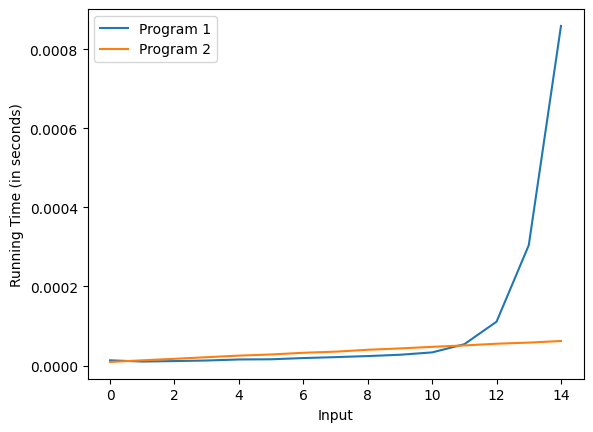
\includegraphics[width=0.75\linewidth]{running_times.png}
        \caption{Runtimes of programs 1 and 2}
        \label{fig:enter-label}
    \end{figure}
    Program 1 runs faster on inputs $N < 11$, whereas Program 2 runs faster on inputs $N > 11$ (visually, they seem to have equal runtimes at $N=11$). \\
    
    \item Explain the discrepancies you see between Parts~\ref{itm:RAMtime} and \ref{itm:realtime}.  (Hint: What do we know about the relationship between the RAM and Word-RAM models, and why is it relevant to how efficiently the Python simulation runs?) \\

    The glaring discrepancies are that the runtime of program 1 no longer maintains its linear form in $N$ or strict speed advantage over program 2, in fact getting \textit{much} slower, for $N > 11$. These discrepancies occur because, in reality, computers struggle when handling overly large numbers. This is reminiscent of the relationship between the RAM and Word-RAM models, which are similar but different because the Word-RAM model addresses the elephant in the room of each memory slot in reality having a finite number of registers (bits) that can store numbers up to size $2^w - 1$ ($w$ is the "word-length," or number of registers in each memory slot). We haven't cracked the infinite hardware glitch yet! \\

    The Word-RAM model having a maximum number for memory length and assignment of a constant to a variable is relevant to the Python simulation because, in practicality, Python can't store infinitely large numbers in one space of memory either. When Python tries handling numbers bigger than it can store in one memory slot, the process of accessing them becomes more complicated by requiring the program to check multiple memory locations that each contain chunks of the numbers (instead of one slot had there been infinite registers). Practically, multiplication doesn't take a constant number of steps either as we're multiplying numbers of very large sizes due to the access workarounds and iterations done over each digit of the super long factors (kind of like how it takes humans more time to compute larger and larger products). For these reasons, a Python simulation would have a runtime differing from the theoretical expectation when it has to make accomodations for handling numbers greater than its supposed maximum "word," similar to how a Word-RAM program would take extra steps to deal with upper-bounding sums or products greater than $2^w - 1$. \\

    Relating the previous paragraph back to the programs above, I'd like to highlight how very large numbers tie-in with what each programs does. Program 1 calculates and outputs $13^{2^N + 1}$, which becomes a super large number approaching infinity as $N \rightarrow \infty$. Program 2 calculates and outputs $13^{2^N + 1}$ mod $2^{32}$, which can also be a very large number but has an upper bound of $2^{32} -1$ even as as $N \rightarrow \infty$ due to the modulo being done. Thus, program 1 starts to perform awfully as we see in the runtime graph for large $N$ because the numbers become too large for the python simulation to store or multiply efficiently (AKA, they're longer than Python's analog to Word-RAM's $2^w - 1$. Program 2 maintains its performance with linear runtime for larger $N$ than program 1 due to the upper bound on the numbers it stores and multiplies. Program 2's upper bound of $2^{32} -1$ must be smaller than Python's analog to Word-RAM's $2^w - 1$, otherwise the program's actual runtime would've also diverged from its theoretical expectation over the range of $N$ seen in the runtime graph. \\
    
    \item (optional\footnote{This problem won't make a difference between N, L, R-, and R grades.}) Give a theoretical explanation of the shapes of the runtime curves you see in Part~\ref{itm:realtime}, by providing explicit formulas for the asymptotic runtimes of the two programs (in clock time). You may need to do some research online and/or make guesses about how Python operations are implemented to come up with your estimates. \\

    For this part, I researched a bit into what Python does when handling numbers that exceed the size storable in a "standard machine word," which has either 32 or 64 bits (registers) in most computers. It turns out that numbers bigger than $2^c - 1$, where $c$ is the number of registers in a computer's "standard machine word," get promoted to \textbf{bignums}, or numbers whose digits are typically stored in either base $2^{15}$ or $2^{30}$ using an array of machine words.
    When multiplying bignums, Python continues to use approaches like Grade-School Multiplication (an $O(n^2)$ operation) for small bignums or improved approaches like Karatsuba Multiplication (an $\approx O(n^{1.585})$ operation) and Toom-Cooke Multiplication (an $\approx O(n^{1.465})$ operation) for larger bignums. $n$ in these runtimes represents the number of \textit{machine words} (AKA components of the bignums) being multiplied.\\

    Judging the graph of the runtimes in (b), program 1's curve seems to take almost a parabolic shape as it starts dealing with bignums that are the consequence of using larger $N$ values. Thus, I'd guess that the runtime (in clocktime) of program 1 takes functional form close to: \\
        
        \[
        T_{prog1}(N) =
        \begin{cases} 
            aN + b & \text{if } N \leq 11 \\
            dN^2 + d& \text{if } Z > N > 11 \\
            eN^{1.465} + f& \text{if } N \geq Z
        \end{cases}
        \] \\

        where a, b, c, d, e, f are constants and Z is an arbitrarily large number marking the value of $N$ that establishes large bignums in the python simulation. I assumed the use of Toom-Cooke multiplication on large bignmums just as an example for what the runtime could be for large bignums. I'd like to clarify that since $N$ is discrete, we'll only get runtimes for natural number inputs. The line segment connectors between discrete $N$ values seen on program 1's curve above purely exist so the graph gives the illusion of continuity (and doesn't look weird) even though the points between the discrete $N$ values aren't valid $(N, T(N))$ pairs. \\

    Looking at program 2's curve, I'd guess that the runtime (in clocktime) of program 2 takes functional form close to:

        \[
        T_{prog2}(N) =
        \begin{cases} 
            gN + h & \text{if } N \leq Z \\
            iN + j& \text{if } N > Z\\
        \end{cases}
        \] \\

        where g, h, i, j are constants (with $g > a$, $h > b$, $g \geq i$, and $h \geq j$) and Z is a large number marking the value N would need to take to be stored as a bignum. Still, I think handling the large $N > Z$ would keep the runtime linear (and purely add a constant number of steps to access/handle it as a bignum) because $N$'s value is stored in a counter that doesn't get multiplied by anything. In general, program 2, just never multiplies numbers as large as program 1 does due to its implementation of divisions by $W = 2^{32}$. Thus, we don't have to call a multiplication method with a runtime exponential in $N$ even once our $N$ is a bignum.  

\end{enumerate}

\item (Simulating Word-RAM by RAM) For every Word-RAM program $P$, there is a RAM program $P'$ that simulates $P$ in the sense that:
\begin{enumerate}
    \item $P'$ halts on $(w,x)$ iff $P[w]$ halts on $x$, and 
    \item If $P[w]$ crashes, then $P'$ halts with $\outputpointer=\outputlen=0$. (We are using this output setting to indicate \crash, since the RAM model does not have any crashing in its semantics.)
    \item If $P[w](x)$ halts without crashing, then the output of $P'(x,w)$ equals the output of $P[w](x)$.
     Furthermore,   
       $$\Time_{P'}(x) = O\left(\Time_{P[w]}(x)+n+w\right),$$
where $n$ is the length of $x$.

(This was stated without proof in Lecture Notes 8.) 

\end{enumerate}

Your proof should use an {\em implementation-level} description, similar to the proof that RAM programs can be simulated by ones with at most $c$ registers in Lecture 7.  Recall that Word-RAM programs have a finite but changing memory size $S$ and a read-only variable $\wordlen$; you may want to start your simulation by calculating $S$ and $2^{\wordlen}$.  Then think about how each operation of a Word-RAM program $P$ can be simulated in a RAM program $P'$, taking care of any differences between their semantics in the Word-RAM model vs. the RAM model. Don't forget MALLOC! \\

\begin{center}
\textbf{    Roadmap:}
\end{center} \\

Since this proof used implementation-level description, I'll divide it up by the order of what we'd need to do to implement a Word-RAM simulation with RAM. We need to handle initialization, operations, crashes, and outputs (technically a subportion of operations but I separated it out to highlight the points we want to prove). Runtime analysis at the end will wrap together the claim in (c) as well. \\

\begin{center}
\textbf{    Initialization:}
\end{center} \\

Initialization is the first high-level step of simulating a Word-RAM $(P)$ program with a RAM program $(P')$. It makes sure the RAM program becomes conscious of the Word-Ram's inherent memory-related constraints on number sizes to $2^w -  1$, with $w$ being the word length (number of "registers" in each slot of memory used). \\

Now let's go into the low level details of initialization. We should begin by storing the maximum number that would've been available in the Word-RAM program. Given a word length $w$ that constrains the number of bits in a memory slot for $P[w]$, let this constant be represented by the variable $maxnumber = 2^w - 1$ (which we obtain in $P$ using a $bignum = two \times bigum$ multiplicative loop bound by GOTO commands on if $counter == 0$ and $zero == 0$ for some counter decreasing from an initial constant $w$ and assigning variables $one = 1$ and $two = 2$). Then, consider our input $x$ that takes up size $S = n$ slots in the memory array $M$. We need to ensure that $n < maxnumber + 1$, so we check if $temp = maxnumber + one - n$ is equal to 0. If so, we make $P'$ crash to simulate the crash that would happen in $P[w]$ due to the existence of inaccessible slots in $M$ that no $var = c$ could index since $c < 2^w$ for noncrashing programs $P$. We subsequently need to ensure that no element $x[i]$ for $i \in [n]$ stores a value $> maxnumber$, so we go through each $x[i]$ (using a loop made of GOTO commands on $counter == 0$ and $zero == 0$ for some counter decreasing from an initial constant $n$) and calculate $temp = maxnumber + one - x[i]$ . If $temp == 0$, we make $P'$ crash to simulate the crash that would happen in $P[w]$ where there's a value being stored above the word size. \\

The runtime of initialization is of the order of the "preprocessing" done by $P'$ to crash on inputs that would've crashed $P[w]$. Step 1, calculating $2^w - 1$, takes $w$ complete loops using GOTOS on a diminishing counter earlier initialized and a constant number of steps in each loop to calculate 2 to the power of $w$ – the current counter value, thus making it an $O(1) + O(w) \cdot O(1) = O(w)$ operation. The first crash detecting step, checking whether $n < maxnumber + 1$, takes a constant number of steps using assignment to constants and a GOTO if $temp = maxnumber + one - n == 0$, thus making it an $O(1)$ operation. The second crash detecting step checks whether each $x[i]$ is a value $\leq 2^w - 1$, taking up to $n$ complete loops using GOTOs on a diminishing counter and constant number of steps in each loop to create a temporary variable that will be compared to zero to determine crashes, thus making it an $O(n) \cdot O(1) = O(n)$. Overall, the initialization process needed for $P'$ to simulate $P[w]$ has the worst case runtime of $O(w) + O(1) + O(n)$ operations, leading $P'$ to take extra runtime in order $O(n + w)$ that $P[w]$ wouldn't have had to. \\

\begin{center}
\textbf{    Operations:}
\end{center} \\

Modifying operations as necessary is the second high-level step of simulating $P$ with $P'$, as we need to make sure that every operation in the Word-RAM model can be mimicked identically by the RAM model. Now, I'll dive into the lower-level details of the important buckets of operations we want to implement in our RAM program that are functionally what they would've been in a Word-RAM program.

\begin{enumerate}
    
\item Assigning a constant to a variable ($var = c$): this process takes the same amount of steps in $P'$ and $P[w]$ for valid constants $c \leq maxnumber$. For other values of $c$, we must simulate the crash that $P[w]$ would've had by using a GOTO the command line heading the crash simulation block if a temporary variable $temp = maxnumber + one - var == 0$. This check adds $O(1)$ time to constant assignment in $P'$ that wasn't necessary for $P[w]$. \\

    \item Arithmetic:\\

Results from arithmetic in Word-RAM have the same lower bound as in RAM, which is 0. However, numbers in Word-RAM are uniquely constrained to an upper bound of $maxnumber$ (defined in initialization) due to the $w$ finite number of registers in each memory slot of M. Only addition and multiplication must be altered in $P'(w, x)$ to accommodate for this constraint because, assuming there exist variables whose natural number assignments commands didn't crash the program, addition and multiplication are the sole RAM operations that could output a number $ > maxnumber$. In these cases, we cap off the sum or product at $maxnumber$. \\
    \begin{enumerate}
        \item Addition: for any two variables we desire to add, $var1$ and $var2$, store $sum = var1 + var2$. Then, calculate $temp = maxnumber + one - sum$. Then, we GOTO a command line that assigns $sum = maxnumber$ if $temp == 0$. Overall, modifying addition to upperbound sums takes a constant number of steps and requires an "extra" $O(1)$ steps in $P'$ that weren't needed in $P[w]$. \\
        \item Multiplication: for for any two variables we desire to multiply, $var1$ and $var2$, store $product = var1 \times var2$. Then, calculate $temp = maxnumber + one - product$. Then, we GOTO to command line that assigns $product = maxnumber$ if $temp == 0$. Overall, modifying multiplication to upperbound products takes a constant number of steps and requires an "extra" $O(1)$ steps in $P'$ that weren't needed in $P[w]$ \\
    \end{enumerate}
    
\item Reading/Writing to memory: reading and writing to memory are identical operations in Word-RAM and RAM, so $P'(w, x)$ \textit{would not need to take any extra steps to read or write to memory} that $P[w]$ wouldn't have. This is because reading and writing simply requires us to access a location in memory and either extract the variable there or set it to a different variable, respectively. We can only check $M[i]$ for valid indexes $i \leq n \leq 2^w - 1$ in memory, otherwise $P'$ would've already crashed trying to assign a constant $c > maxnumber$ to $i$, so $P$ and $P'$ will read/write identically because there's no additional constraints on that in the Word-RAM model once we're certain all numbers fall within the aforementioned bounds. \\

\item MALLOC: MALLOC in $P'$ will be carried out similary to $P[w]$, but we must consider when allocating new memory for our array M that it must all be accessible for reading/writing. Since our maximum number is $maxnumber$, the size of M must be $\leq maxnumber$ because no valid constant could be assigned to variables that let us access $M[maxnumber:]$. Thus, with each MALLOC call, we must calculate $temp = S$, where $S$ is the size of our memory array M that was initially equal to $n$, the size of our input array $x$. Then, we we let $temp = maxnumber + one – temp$ and GOTO a command line heading a block (described in the crash section below) that causes $P'$ to simulate crashing if $temp == 0$. Overall, MALLOC in $P'$ takes a constant number of steps to allocate an additional memory slot to M and a constant number of steps to ensure the updated size of M would not crash $P[w]$. The size check needed during each MALLOC call makes $P'(w, x)$ take $O(1) = O(1)$ extra steps that wouldn't have been needed in $P[w]$ when calling MALLOC. \\
\end{enumerate}


Overall, operations in $P'$ require on the order of $O(1) + O(1) + O(1) + O(1) = O(1)$ extra steps to simulate Word-RAM operations that wouldn't have been necessary in $P[w]$.

\\

\begin{center}
  \textbf{  Crashes \\}
\end{center}

To be thorough according to my implementation of a crash in $P'$, I'd like to clarify that the crash checks mentioned will \textit{ALL} GOTO the start of a block of command lines assigning $\outputpointer= 0, \outputlen=0$, and returning $M[\outputpointer: \outputpointer + \outputlen - 1] = M[0:-1]$ in the case of a crash per the question's request. A Word-RAM program only crashes when a number in the input array $x$, the size $S$ of the memory array M, or one of the constants $c$ in assignment commands ($var = c$) exceeds $maxnumber$. I've framed how $P'$ addresses each of these conditions in my preceding implementation, which generally involves checking the zero identity on various crash indicator variables to GOTO to the start of the crash simulation command lines illustrated at the start of this section. Implementing the "crash" feature in $P'$ to simulate the crashes occurring in $P[w]$ purely adds a constant number of steps to the initialization condition or operation that the crash is associated with. It's constant runtime due to the constant number of lines in the crash command block that we GOTO if $indicator == 0$, thus making simulating a crash take $O(1)$ extra steps in $P'$ that wouldn't have been necessary in the Word-RAM program (it would've just immediately crashed). \\

\begin{center}
\textbf{    Output:}
\end{center} \\

The output returned for $P'$ on $P[w]$ that halts with an output is $M[\outputpointer : \min(\outputpointer + \outputlen - 1, S-1)]$, which exactly matches the Word-RAM program's output that factors in the size constraint on M. Intuitively, that's what we expect in a proper simulation. The "min" term can be found in $O(1)$ steps simply by letting a temporary variable $temp = \outputpointer + \outputlen - one - (S - one)$ and having a GOTO $min = \outputpointer + \outputlen -1$ if $temp == 0$ ($min = S - 1$ is the default ending index we use if the GOTO isn't engaged). By simulating the output structure of $P[w]$ by returning the contents of M from index $\outputpointer$ to the array's end, we effectively make $P'(x)$ return the same output as $P[w](x)$ that halts without crashing as stated in (c.1) $\checkmark$. For $P[w](x)$ that does crash, $P'(x)$ halts on output $M[0:-1]$, which fits the specifications that let the RAM model express crashing some way despite the absence of crashing in its semantics per (b) $\checkmark$. \\ 

$P[w]$ halting on input $x$, either through a crash or returning of an output, thus always means $P'$ halts on $(w, x)$ per my design of the implementation of simulation $P'$ (and the previous proof of parts b, c.1). Conversely, $P'(x)$ halting implies $P[w]$ halts on $x$ because $P[w]$ is fully expressed by $P'$ and must've either crashed if $P'(x) = M[0:-1]$ or returned $M[\outputpointer : \min(\outputpointer + \outputlen - 1, S-1)]$ (the same as $P'(x)$ that halts with output per our proof of (c.1)). Since we've proven the conditional statement and its converse both true through the simulation implementation, the biconditional $\Leftrightarrow$ statement is true (a) $\checkmark$ \\

\begin{center}
\textbf{    Runtime}
\end{center} \\

Throughout the entire implementation, I've been tracking the amount of "extra" steps that it takes to simulate a Word-RAM programs with a RAM program. I'm almost thinking of these "extra" steps like the runtime of pre/postprocessing in a reduction from RAM expressionism to Word-RAM expressionism where the oracle is simply the Word-RAM command line we're aiming to express with RAM commands. These "extra" steps are of the order of the sums of the "extra" steps it takes for initialization, operations, and simulating crashing or returning the same output $P$ would've returned upon halting (assuming $P$ halts as is posed in (c)). That makes the "extra" steps $P'$ takes of order $O(n + w) + O(1) + O(1) = O(n + w)$, and thus proves $\Time_{P'}(x) = O\left(\Time_{P[w]}(x)+n+w\right)$, because the worst case runtime of $P'$ is the worst case runtime of $P[w]$ plus the worst case runtime of the "additional" steps $P'$ must carry out to fully express $P$ using the RAM model (c.2) $\checkmark$. \\


\item (reflection) Discuss the value (or lack thereof) that you think computational models, and the RAM and Word-RAM models in particular, have for computer science.  All opinions are valid, as long as they show serious thought and are backed by specific justifications.

\textit{Note: As with the previous psets, you may include your answer in your PDF submission, but the answer should ultimately go into a separate Gradescope submission form.}

\item Once you're done with this problem set, please fill out \href{https://forms.gle/TG8cG4LWN3S4T6za6}{this survey} so that we can gather students' thoughts on the problem set, and the class in general. It's not required, but we really appreciate all responses!

\end{enumerate}


\end{document}

